% Propósito: enseñar a leer la tendencia de la aproximación lineal de la
% velocidad del sonido con la temperatura ambiental.
% Origen: c=(331+0,6 theta) m/s, ecuación
% \eqref{eq:u2-velocidad-temperatura}. Los puntos son valores calculados del
% modelo, no mediciones. Intervalo representado: 0 a 30 grados Celsius.
% Descripción accesible: un gráfico cartesiano muestra la temperatura entre
% 0 y 30 grados Celsius en el eje horizontal y la velocidad entre 325 y
% 355 metros por segundo en el eje vertical. Una recta ascendente pasa por
% los puntos 331, 337, 343 y 349 metros por segundo para 0, 10, 20 y 30 grados
% Celsius, respectivamente.
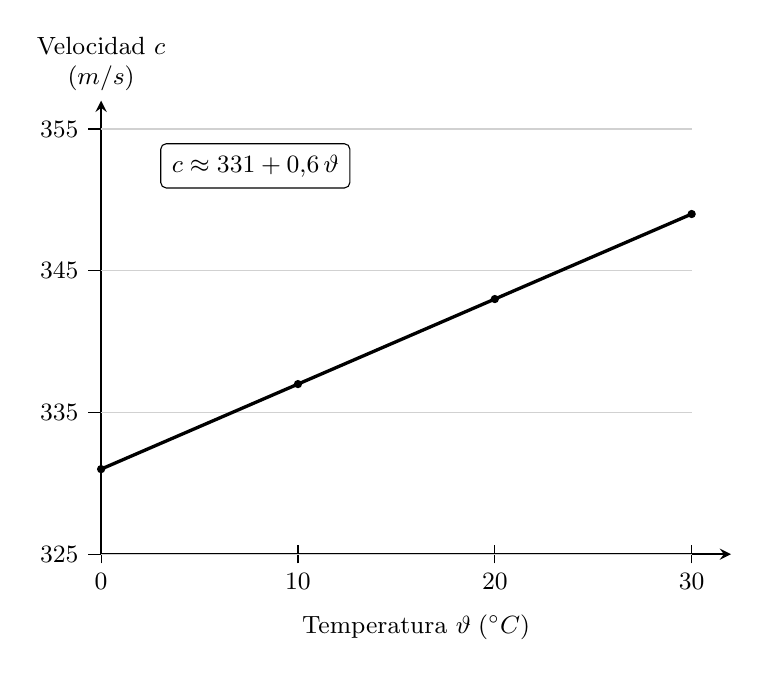
\begin{tikzpicture}[font=\small,>=stealth,x=0.25cm,y=0.18cm]
    % La coordenada vertical representa c-325 para mantener legibles las
    % variaciones dentro del intervalo declarado.
    \draw[->,thick] (0,0) -- (32,0);
    \node[below] at (16,-3.6)
        {Temperatura \(\vartheta\;({}^{\circ}\text{C})\)};
    \draw[->,thick] (0,0) -- (0,32);
    \node[above,align=center] at (0,32)
        {Velocidad \(c\)\\\((\text{m}/\text{s})\)};

    \foreach \temp in {0,10,20,30}{
        \draw (\temp,-0.65) -- (\temp,0.65);
        \node[below] at (\temp,-0.65) {\temp};
    }
    \foreach \vel in {325,335,345,355}{
        \pgfmathsetmacro{\posy}{\vel-325}
        \draw (-0.65,\posy) -- (0.65,\posy);
        \node[left] at (-0.65,\posy) {\vel};
        \draw[black!18] (0,\posy) -- (30,\posy);
    }

    \draw[very thick] (0,6) -- (30,24);
    \foreach \temp/\vel in {0/331,10/337,20/343,30/349}{
        \pgfmathsetmacro{\posy}{\vel-325}
        \fill (\temp,\posy) circle (1.5pt);
    }

    \node[
        draw,
        fill=white,
        rounded corners=2pt,
        inner sep=4pt,
        anchor=north west
    ] at (3,29)
        {\(c\approx331+0{,}6\,\vartheta\)};
\end{tikzpicture}
